% !TEX root =  paper.tex

\subsection{Results and Discussion}\label{sec:discussion}

\begin{figure}[t]
    \centering
    \includegraphics[trim={0.3cm 0.3cm 0.3cm 0.3cm},clip,height=7.9cm, width=0.72\textwidth]{testability/figures/DOM-boxplot.eps}
    \caption{Accuracy of the inferred augmented DOM for each evaluated application in table \ref{table:eval-apps}. A total of 50 canvas elements in five different applications where used for this experiment.}
    \label{fig:result-DOM-accuracy}
\end{figure}

\head{Accuracy}
Figure \ref{fig:result-DOM-accuracy} shows box plots for the accuracy of \tool. 
The x-axis shows our subject applications, and the y-axis shows the  similarity percentage between the original canvas and the canvas regenerated from the inferred augmented canvas DOM. The runtime average for the tool is relatively fast at around 4 $\pm$ 0.3 seconds.

We make a number of observations from Figure \ref{fig:result-DOM-accuracy}. First, we note that most inferred DOMs have an accuracy close to or above $90 \%$ (the average for the dataset is $91.2 \% \pm 1.3$). Furthermore, at the highest and lowest of outliers, the accuracy ranges between $98 \%$ and $85 \%$. Therefore, we conclude from these results that the DOM inference process is relatively accurate in representing the canvas.

As for the accuracy at the lower end of the outliers, the reason for this is the inability of the probabilistic Hough transform used by the algorithm (as described in section \ref{sec:approach}) to generate segments to cover the small boundaries of small objects. These often take the form of small appendages connected to various objects, and the probabilistic Hough transform misses such small appendages. In a future version of the algorithm, we plan to improve the performance by finding a more suitable alternative than the probabilistic transform.

\head{Effectiveness}
Table \ref{tbl:result-fault-injections} shows the effectiveness results for \tool. 
Each row shows the total number of faults injection performed on the application, and then the number of true positives and false negatives reported by \tool, as described in section \ref{sec:experimental-procedure}.

From Table \ref{tbl:result-fault-injections}, we note that the overall rate of detecting true positives is $93\%$ and the overall rate of false negatives is $7\%$. Furthermore, we note that the per-application true positive rate varies from 16 out of 20 ($80\%$, lowest) to 20 out of 20 ($100\%$, highest). 
As such, we conclude from these results that the approach is relatively reliable in detecting faults in canvas elements. 

The main reason for the false negatives is that the probabilistic Hough transform used by the algorithm was unable to generate segments that would cover some of the injected shapes that were small appendages to other objects and this resulted in no modification to the segments set of the object. This is therefore reflected as a false negative. As part of our future improvements, we would like to improve the true positives rate even further by finding a better alternative to the probabilistic transform.

\begin{table}[b]
\setlength{\tabcolsep}{6pt}
\renewcommand{\arraystretch}{0.9}
\centering
\caption{Results of detecting fault injections}
\begin{tabular}{lccc}
\toprule
\textbf{Application} &  \textbf{\# Injections}  &  \textbf{\# True Positives} & \textbf{\# False Negatives} \\
\midrule
JBrowse~\cite{eval_app_jbrowse}      & 20 &  18  &  2 \\
Reactome~\cite{eval_app_reactome}    & 20 &  20  &  0 \\
Scribl~\cite{eval_app_scribl}        & 20 &  16  &  4 \\
Gibberish~\cite{eval_app_gibberish}  & 20 &  19  &  1  \\
iCanplot~\cite{eval_app_icanplot}    & 20 &  20  &  0 \\
\midrule
Total:  & 100   &  $93 \%$ &  $7 \%$ \\

\bottomrule
\end{tabular}
\label{tbl:result-fault-injections}
\end{table}

\head{Threats to Validity}
Our choice of subject applications could be a source of external threat to validity. In order to mitigate this threat, we select subject applications from a wide range of complexity (from around 7,000 to more than 100,000 LOC), and also select the applications from a varying assortment of fields, such as medicine, music, and chemistry. Another related threat is the relatively low number (five) of evaluated subjects. We mitigate this threat by extracting a random collection of 50 canvas snapshots for these applications and running 100 fault injections. \hl{Furthermore, some aspects in the fault injection process could be a source of internal threat to validity. There is currently no compilation of the types of faults that exist for canvases. Accordingly, 
in order to mitigate this threat and have an unbiased fault injection process, we chose to inject random shapes into the canvas. 
We also adopt a uniform approach of consistently injecting random objects on the canvas regardless of the applications's API, as opposed to individually injecting faults by modifying the specific API parameters of each canvas app. This helps in ensuring equally random fault injection across subjects. 
Furthermore, and perhaps most importantly, we do not have access to the objects on the canvas due to the lack of observable state in the canvas, which is the very problem that our approach is trying to solve. Accordingly, due to absence of access to canvas objects, simulating a fault by removing a certain object is not practically achievable.} Another related threat is the possible bias in the determination of true positives or false negatives. We mitigate this threat by injecting faults across all trials and then using a quantitative distance metric with a normalized range to allow a direct binarization of results into true positives and false negatives. 

Another potential threat to validity is the issue of cross-browser compatibility. We note that the rendering of canvas elements is categorically different from rendering regular web pages. When rendering a page, the browser has to continuously maintain a DOM and regularly recompute layout position and visual properties of the page elements before rendering. For canvas, however, the browser does not maintain any layout information about the canvas, and simply paints the pixels from the API call directly on screen. All browsers relay the pixel-by-pixel rendering directly to the canvas. Canvas elements have no observable state and browsers do not participate in maintaining what does or does not get rendered. This is the opposite of rendering webpages.

To the best of our knowledge, there is no evidence in the literature of cross-browser incompatibilities for canvas elements. Furthermore, in a recent study \cite{bajaj2014mining} categorizing questions asked by developers on StackOverflow, canvas related questions were mostly about how to use the canvas API. There was no reported pattern of questions on canvas-related cross browser incompatibility issues. In addition, and more importantly, from our own use and testing of canvas elements, we did not notice incompatibility issues either. For these reasons, we do not consider cross-browser incompatibility to be a threat to the validity of the proposed approach.


